\documentclass[12pt]{article}
\usepackage[utf8]{inputenc}	% Para caracteres en español
\usepackage{amsmath,amsthm,amsfonts,amssymb,amscd}
\usepackage{multirow,booktabs}
\usepackage[table]{xcolor}
\usepackage{fullpage}
\usepackage{lastpage}
\usepackage{enumitem}
\usepackage{fancyhdr}
\usepackage{mathrsfs}
\usepackage{wrapfig}
\usepackage{setspace}
\usepackage{calc}
\usepackage{multicol}
\usepackage{cancel}
\usepackage{enumitem}
\usepackage{pdfpages}
\usepackage{caption}
\usepackage{subcaption}
\usepackage{lastpage}
\setlist{nolistsep}
\usepackage[retainorgcmds]{IEEEtrantools}
\usepackage[margin=3cm]{geometry}
\usepackage{amsmath}
\newlength{\tabcont}
\setlength{\parindent}{0.0in}
\setlength{\parskip}{0.05in}
\usepackage{empheq}
\usepackage{framed}
\usepackage[most]{tcolorbox}
\usepackage{xcolor}
\colorlet{shadecolor}{orange!15}
\parindent 0in
\parskip 12pt
\geometry{margin=1in, headsep=0.25in}
\theoremstyle{definition}
\newtheorem{defn}{Definition}
\newtheorem{reg}{Rule}
\newtheorem{exer}{Exercise}
\newtheorem{note}{Note}

\usepackage[style=numeric,maxbibnames=9,sorting=none]{biblatex}
%\bibliographystyle{IEEEtran}
\addbibresource{references.bib}% Syntax for version >= 1.2

% Increment the page number by 1 before printing it to include titlepage
\newcommand{\totalpages}{\number\numexpr \lastpageref{LastPages} + 1 \relax}


\pagestyle{fancy}
\fancyhf{} % clear existing header/footer entries
% Place Page X of Y on the center
% side of the footer
\fancyhead{}
\renewcommand{\headrulewidth}{0pt}
\fancyfoot[C]{Page \textbf{\thepage} of \textbf{\pageref{LastPage}}}

\makeatletter
\renewenvironment{titlepage}
 {%
  \if@twocolumn
    \@restonecoltrue\onecolumn
  \else
    \@restonecolfalse\newpage
  \fi
  \thispagestyle{empty}%
 }
 {%
  \if@restonecol
    \twocolumn
  \else
    \newpage
  \fi
 }
\makeatother


\begin{document}

\begin{titlepage}
\thispagestyle{fancy}
   \begin{center}
       \vspace*{1cm}
       
\includegraphics[width=4cm]{plots/color-center-UWlogo-print.png} \\
       Fall 2023 ME/CS/ECE759 Final Project Report\\
       University of Wisconsin-Madison

       \vspace*{4cm}

       {\Huge \textbf{Parallel Implementation of Coordinated Animal Motion}}
            
       \vspace{1.5cm}

       \textbf{Rutwik Jain, Neeraj Surawar}\\
       \{rnjain, surawar\}@wisc.edu

       \vfill
    
        
       {\Large December 13, 2023}
        \vspace{0.8cm}
            
   \end{center}
\end{titlepage}

\newpage
\begin{center}
    {\Large \textbf{Abstract}}

The text of the abstract comes here. Should be about half page, like a summary of what was proposed and what has been accomplished.

Link to Final Project git repo: dropthelinkhere



COMMENTS (remove this highlighted stuff when you submit your Final Project PDF report):
Drop this Final Project PDF report in Canvas in the folder “FinalProject759” by December 13,
2023, at 9 PM. Use font size 12 throughout the document. Do not go beyond 10 pages unless you really
feel you have to (page count doesn’t include TOC, abstract, etc.). Feel free to use a LaTeX source as
long as you follow this format; in the end, you will be uploading a PDF anyway.
Please stick with the Sections and section titles provided. It simplifies your life and ours.
Please make sure that you include in this *abstract* a link to the git repo for your project (see the text
highlighted red above). Using this link (i) we will clone your project repo; (ii) we will look at the
progress history for your project as documented by git.
To verify that you provided the right git link, click on it. It should take you to your git repo.
Finally, please make sure the TAs and Dan are added as a collaborators to your git repo, so that we can
clone your repo.

\end{center}

\newpage
\renewcommand{\baselinestretch}{0.2}\normalsize
\tableofcontents
\renewcommand{\baselinestretch}{1.0}\normalsize

\newpage
\section{General Information}
\begin{enumerate}
    \item Name: Rutwik Jain
    \item Email: rnjain@wisc.edu
    \item Home department: Computer Sciences
    \item Status: PhD Student
    \item Teammate: Neeraj Surawar (Yes, the report is identical to this)
    \item I release the ME759 Final Project code as open source and under a BSD3 license for unfettered use of it by any interested party.
\end{enumerate}

\section{Problem Statement}
Aggregate, coordinated motion of bodies, such as a flock of birds, school of fish or herd of animals commonly occurs in nature (Figure~\ref{fig:intro}). Creating such flocking behavior in simulation is also a well-studied problem in computer graphics. In a SIGGRAPH paper in 1987~\cite{cr-siggraph}, Craig Reynolds first defined the term ``boid flocking" to refer to such flocking behavior, where ``boid" refers to each independent actor that works in coordination with others to produce the overall flocking effect. His work~\cite{cr-siggraph} also produced a behavioral model and physics-based simulation of such flocking. In this 

\begin{figure}[ht!]
\centering
    \begin{subfigure}[t]{0.45\textwidth}
        \centering
        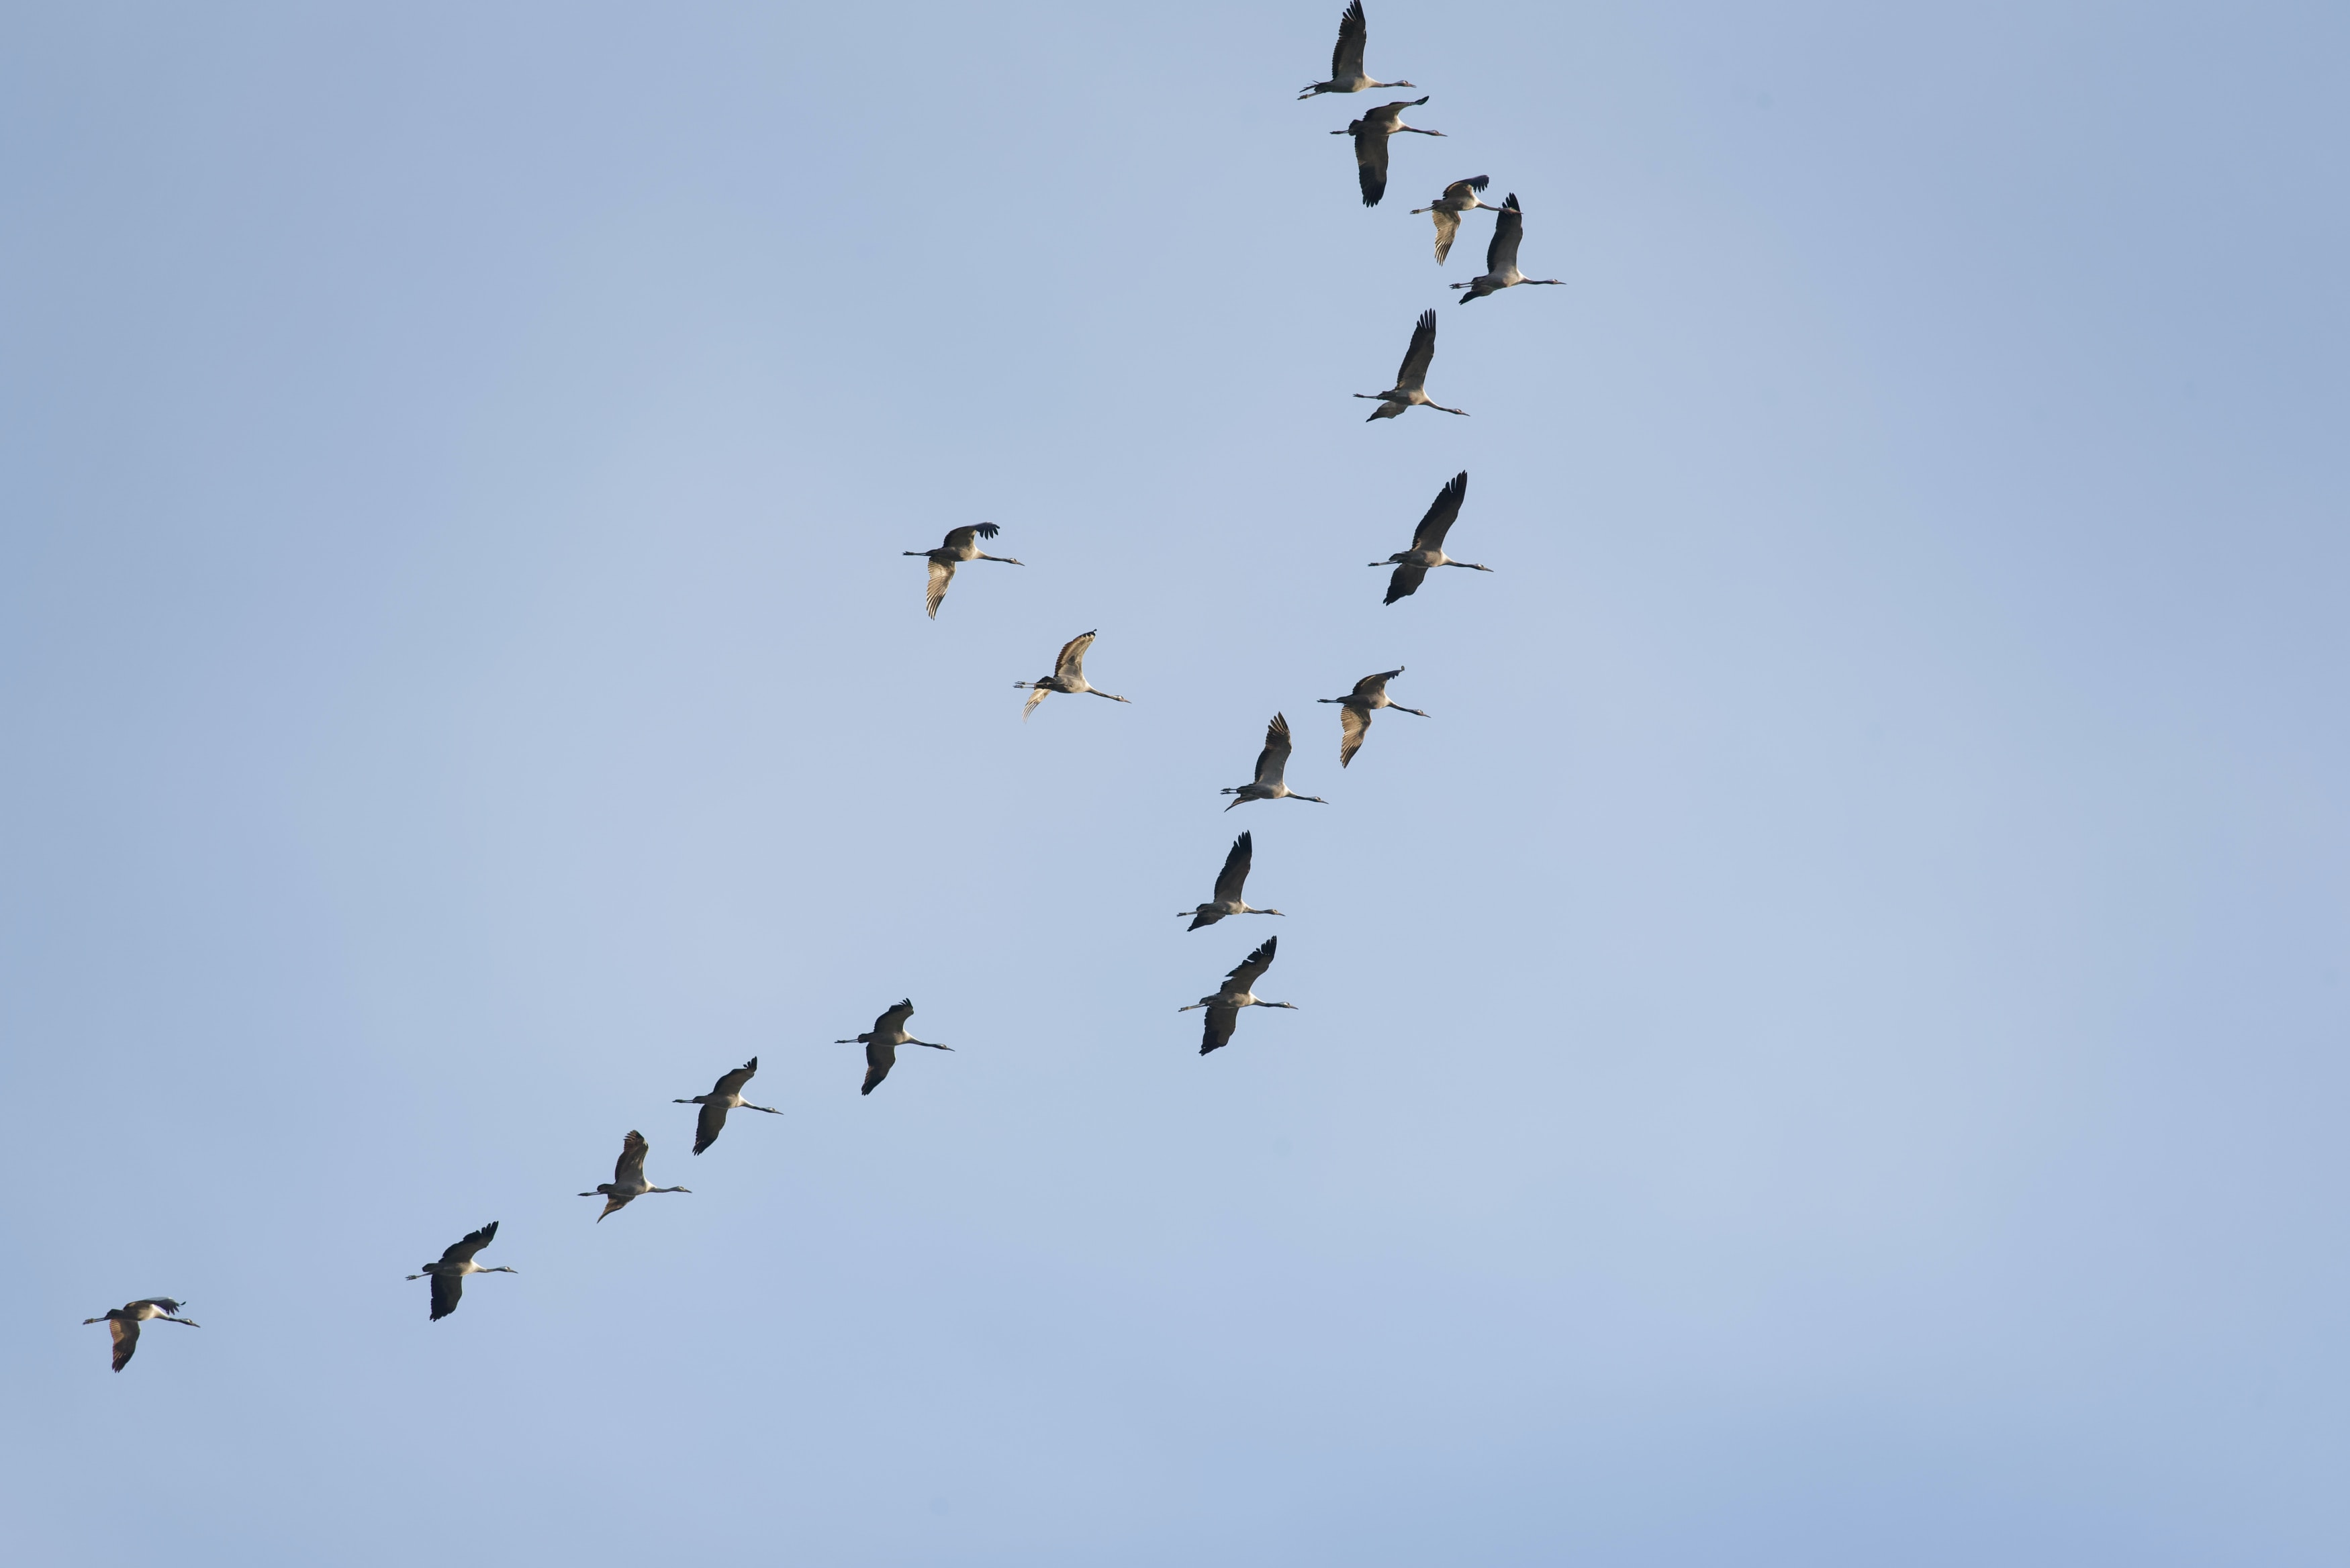
\includegraphics[scale=0.059]{plots/migrating-cranes.jpg}
        \caption{Migrating cranes (Photo by REGINE THOLEN on Unsplash)}
    \end{subfigure}
    \hfill
    \begin{subfigure}[t]{0.45\textwidth}
        \centering
        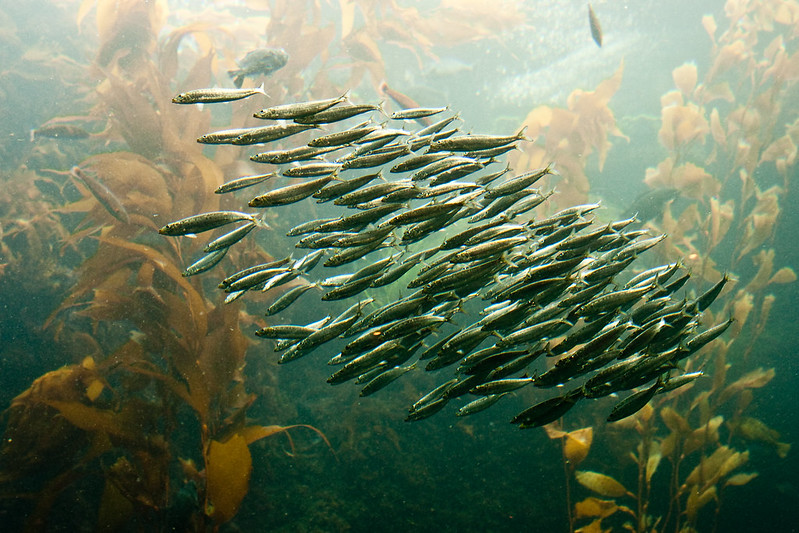
\includegraphics[scale=0.26]{plots/school-of-fish.jpg}
        \caption{School of fish (Creative commons license, Flickr)}
    \end{subfigure}
    \caption{Examples of flocking behavior in nature}
    \label{fig:intro}
\end{figure}

\input{sections/02_Solution}
\newpage
\section{Overview of Results. Demonstration of Project}
% 
Show gif/PPM sequence to demonstrate flocking 

% 
Talk about variable parameters \\
\texttt{
num\_boids \\
perception\_radius \\
num\_threads \\
}

% Per-frame latency 
Figure~\ref{fig:framelatency} shows the latency incurred in performing computations and rendering each frame for a simulation of 1000 frames with varying number of boids. For a given simulation, the plot shows that per-frame latency is fairly consistent over time, and flocking performance can therefore be evaluated using average metrics such as frame rate (FPS). The plot also shows that naïve CPU-based boid-flocking scales poorly with increasing number of boids.

\begin{figure}[ht!]
\centering
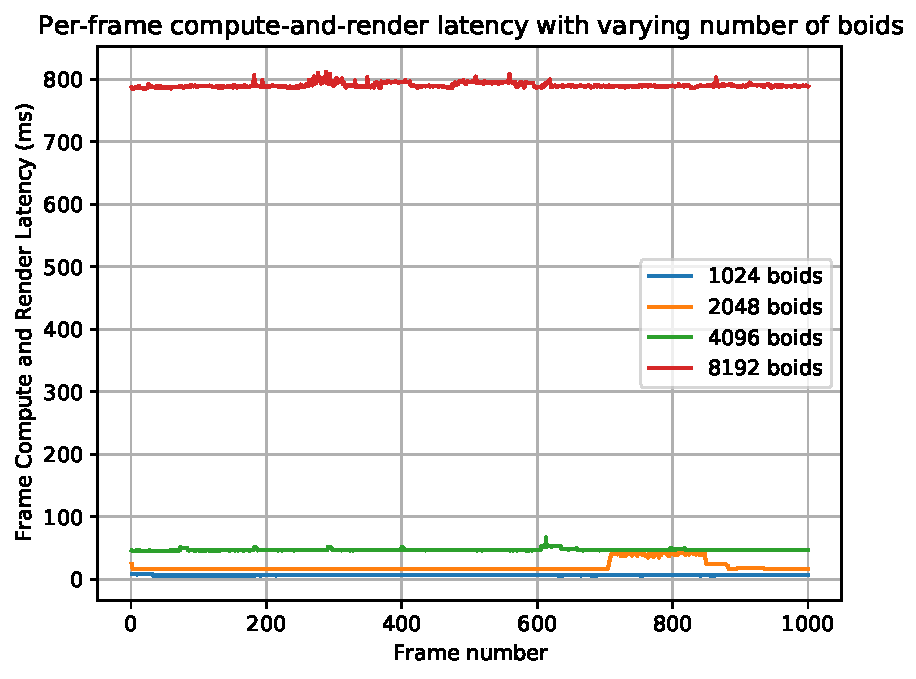
\includegraphics[scale=0.8]{plots/latency-per-frame.pdf}
\caption{Time taken to compute and render each frame in milliseconds for a naïve CPU-based implementation.}
\label{fig:framelatency}
\end{figure}

\section{Deliverables: Building \& Running the Project}



\section{Conclusions and Future Work}


\printbibliography

\end{document}